%*******************************************************************************
%****************************** Fourth Chapter *********************************
%*******************************************************************************

\chapter{Discussion}

\ifpdf
    \graphicspath{{Chapter7/Figs/Raster/}{Chapter7/Figs/PDF/}{Chapter7/Figs/}}
\else
    \graphicspath{{Chapter7/Figs/Vector/}{Chapter7/Figs/}}
\fi

\section{zEdge segmentation results}

\begin{figure}[htbp!]
\centering
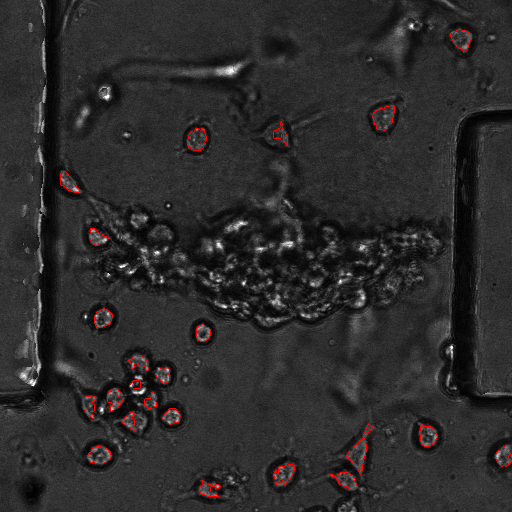
\includegraphics[width=1.0\textwidth]{5224-zedge_seg-tile_050714_s13_ch-zbf-8-5-5-outline-zcomp-8-1-1-zedge-8-5-5-TYOGE5XI_t0}
\caption{zEdge segmentation}
\label{fig:zedge_segmentation}
\end{figure}

Several cells in Figure~\ref{fig:zedge_segmentation} were mis-recognised. The cell in the centre of the group on the lower left is a good example. The mis-recognition in this case is due to bright flecks in the interior of the cell that prevent the segmentation from extending from the marker to other locations in the interior. This could be ameliorated by selectively smoothing the Brightfield inside the edges. Unfortunately, this process would also dampen the appearance of other parts of the cells, such as protrusions, that have poorly defined edges. An analogous situation occurs in GFP images~\cite{arce}.

Another mis-recognition occurs in the cell at the top of the image in the centre of the group of three. This does not appear to be a result of highly non-uniform interior, but the segmentation algorithm did not allow the recognition to continue. This can be improved by increasing the contrast between the cell interior and the background, causing the cell interior to appear to be of higher value than the background and allowing the segmentation to continue.

In general, mis-recognition occurs when there is no clear reason for the segmentation to continue. This is also dependent on the starting location of the marker in the Brightfield. Another starting location with a higher intensity will be more likely to fill the lower intensities around it.

\section{zMod sensitivity results}

We expected that the correspondence between the manual segmentation ground truth and the zEdge segmentation would increase when the noise was reduced (by increasing $\Sigma$). Increasing R (the size of the mask used to produce the GFP pixel profile for each x-y position) was expected to mix the z-levels in neighbouring pixels to make contiguous regions of similar z-levels more uniform. This was observed in the resulting images.

However, neither increased R nor increased $\Sigma$ had significant effect on the Fscore of our preprocessed images. We had thought that smoother, less noisy images would produce more accurate segmentation, but this is contradicted by the Fscore results. The method itself, however, still yields higher Fscores than the method described by Selinummi et al.

\section{Comparison of preprocessing methods}

\begin{figure}[htbp!]
\centering
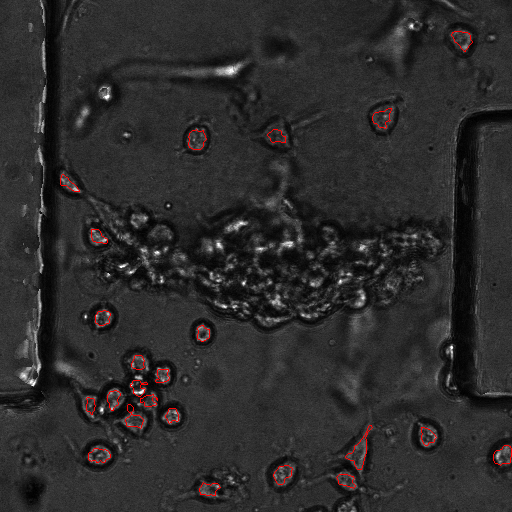
\includegraphics[width=1.0\textwidth]{5223-bf_std_seg-tile_050714_s13_ch-zbf-8-5-5-outline-zcomp-8-1-1-bmod-PLG5WADE_t0}
\caption{BPP segmentation}
\label{fig:bmod_segmentation}
\end{figure}

Both segmentation results in Figure~\ref{fig:zedge_segmentation} and Figure~\ref{fig:bmod_segmentation} do fairly well at picking up the general shape of the cells.

Our segmentation more consistently approximates the dark Brightfield edges. It appears as though the Selinummi method compresses the segmentation; its resulting edges lie away from the true edges. It instead produces edges that are closer to the interior of the cell. This probably explains the decrease in Fscore for this method.

The regions assigned a higher contrast by the Selinummi method have highly variable Brightfield profiles in the z-dimension. In the Brightfield data, the locations of the true edges will not have highly variable profiles. Instead, the regions immediately on either side of the edge will be the most highly variable, as these are where Brightfield intensity discontinuities actually occur. The Selinummi method looks for this disturbances in order to find cell edge pixels. This causes a systematic underestimation of the extent of the cell. In contrast, our method use GFP intensity pixel profiles to select an image section from the Brightfield stack for each cell pixel or group of cell pixels. We thus preserve the darker edges and strengthen them.
